\documentclass[12pt]{article}
\usepackage[utf8]{inputenc}
\usepackage[a4paper, margin=2cm]{geometry}
\usepackage[T1]{fontenc}
\usepackage{graphicx}
\usepackage{geometry}
\usepackage{amsmath}
\usepackage{amsfonts}
\usepackage{amssymb}
\usepackage{booktabs}
\usepackage{hyperref}
\usepackage{fancyhdr}
\usepackage{float}
\usepackage{ulem}
\usepackage{xeCJK}
\usepackage{listings}
\usepackage{xcolor}
\usepackage{indentfirst}
\setmainfont{Times New Roman}
\setCJKmonofont[BoldFont=SimHei, AutoFakeBold=true]{SimSun}
\lstset{
    basicstyle=\ttfamily\small,
    commentstyle=\color{gray},
    keywordstyle=\color{blue},
    stringstyle=\color{red},
    numberstyle=\tiny\color{gray},
    breaklines=true,
    captionpos=b,
    keepspaces=true,
    numbers=left,
    numbersep=5pt,
    showspaces=false,
    showstringspaces=false,
    showtabs=false,
    tabsize=2,
    frame=single,
    language=[x86masm]Assembler
}

\begin{document}
\thispagestyle{empty}

\begin{center}
    \vspace*{2cm}
    
    \Huge \textbf{2023-2024学年春季学期} \\
    \vspace{2cm}
    
    \Huge \textbf{《汇编语言程序设计》} \\
    \vspace{4cm}
    
    \large 评分：\underline{\hspace{4cm}} \\
    \vspace{6cm}
    
    \begin{tabular}{rl}
        \Large 学\hspace{2em}院： & \Large \underline{\makebox[12em][l]{\quad 计算机科学与工程学院}} \\
        \Large 专\hspace{2em}业： & \Large \underline{\makebox[12em][l]{\quad 计算机科学与技术}} \\
        \Large 班\hspace{2em}级： & \Large \underline{\makebox[12em][l]{\quad 计算机2204班}} \\
        \Large 姓\hspace{2em}名： & \Large \underline{\makebox[12em][l]{\quad 李俊洁}} \\
        \Large 学\hspace{2em}号： & \Large \underline{\makebox[12em][l]{\quad 20225443}} \\
        \Large 任课教师：         & \Large \underline{\makebox[12em][l]{\quad 刘思宇、柳秀梅}} \\
    \end{tabular}
    \vfill
\end{center}
\newpage

\section{实验目的}
本实验的主要目的是通过汇编语言编程来加深对程序模块化设计和子程序调用机制的理解。
通过具体的编程任务，学习如何设计和实现子程序来完成特定的功能，如计算多字节数据的绝对值和两个数据的和。实验通过操作实际的数据来掌握这些基本概念和技巧，进一步提高问题分析与解决能力以及汇编语言的应用能力。

具体的学习目标包括：
\begin{itemize}
    \item 学习如何在汇编语言中设计和实现功能性的子程序。
    \item 掌握子程序调用的方法以及参数的传递方式。
    \item 通过实践加深对汇编程序中地址指向、数据处理和循环控制的理解。
    \item 实践中学习如何处理多字节数据和进行数值的绝对化处理。
    \item 理解并实现两组数据之间的算术运算，深入学习程序的模块化和代码重用。
    \item 提升程序调试能力，通过错误分析和修改来验证程序的功能和效率。
\end{itemize}

\section{实验要求}
本实验要求学生能够熟练地应用汇编语言进行程序设计，并通过具体的编程任务，深入理解子程序的设计与实现。
实验要求如下：
\begin{itemize}
    \item 模块化设计：程序需要分模块编写，主要功能分别用子程序实现，包括求绝对值和求和操作。
    \item 数据处理：正确处理内存中的多字节数据，并能够通过子程序对这些数据进行操作。
    \item 子程序实现：实现两个子程序，一个用于计算多字节数据的绝对值，另一个用于计算两个多字节数据的绝对值之和。
    \item 测试验证：通过不同的数据组合进行测试，确保程序在各种情况下都能正确运行并得到预期结果。
    \item 文档和注释：源代码需要有详细的注释，实验报告中需包括对子程序设计和主程序流程的详细描述。
\end{itemize}

\section{实验内容}
已知两个长度相等的带符号的多字节数据分别存放在内存DATA1和DATA2开始的连续单元中，数据长度存放在LEN单元。
编制程序，计算两个数据的绝对值之和，将结果存放在SUM开始的连续单元中。

求一个多字节数据的绝对值及求两个多字节数据的和的功能分别用子程序来实现；

分别用三组数据调试程序，检验程序的正确性：
\begin{itemize}
    \item 两个多字节数据都是正数；
    \item 两个多字节数据都是负数；
    \item 两个多字节数据一正一负。
\end{itemize}
\section{源程序}
    \begin{lstlisting}[caption={汇编源代码}, label=lst:asm2]
dseg    segment
    data1   db 1, 2, 3, 4, 5, 6, 7, 8, 9, 10
    data2   db 1, 3, 5, 7, 9, 11, 13, 15, 17, 19
    ; data1   db -1, -2, -3, -4, -5, -6, -7, -8, -9, -10
    ; data2   db -1, -3, -5, -7, -9, -11, -13, -15, -17, -19
    ; data1   db 1, -2, 3, -4, 5, -6, 7, -8, 9, -10
    ; data2   db 1, -3, 5, -7, 9, -11, 13, -15, 17, -19
    len     db 10
    sum     db 0, 0, 0, 0, 0, 0, 0, 0, 0, 0
dseg    ends

sseg    segment  stack
    stack   db  100h  dup  (?)
sseg    ends

cseg    segment
    assume cs:cseg, ds:dseg, ss:sseg
start:
    mov  ax, dseg               ; 初始化
    mov  ds, ax
    mov  ax, sseg
    mov  ss, ax
    mov  sp, 100h

    lea  di, data1              ; di存data1
    call my_abs                ; 调用绝对值处理程序处理data1
    lea  di, data2              ; di存data2
    call my_abs                ; 调用绝对值处理程序处理data2

    lea  di, data1              ; di存data1
    lea  si, data2              ; si存data2
    lea  bx, sum                ; bx存sum
    call add_seg

    mov  ah, 4ch                ; 结束程序
    int  21h

; 绝对值计算子程序
; 输入: di作为字段的起始地址，中途会使用到cx
; 输出: di位置改变
; 修改: 字段元素将被替换为绝对值
my_abs proc near
    xor  ch, ch                 ; ch清零
    mov  cl, [len]              ; 数组长度
do_abs:  
    cmp  byte ptr [di], 0       ; 与0比较
    jge  is_positive            ; 正数或0
    neg  byte ptr [di]          ; 负数取补
is_positive:
    inc  di                     ; 下一个地址
    loop do_abs                ; 循环执行，用len控制循环次数
    ret
my_abs endp

; 加法计算子程序
; 输入: di数组1起始地址, si数组2起始地址，bx为输出数组的起始地址，中途会使用到al、cx
; 输出：bx为数组1加数组2的起始地址
; 修改：bx为输出数组、di、si数组内容被修改
add_seg proc near
    xor  ch, ch                 ; ch清零
    mov  cl, [len]              ; 数组长度
do_add:
    mov  al, byte ptr [di]      ; 从di指向的地址加载
    add  al, byte ptr [si]      ; 相加
    mov  [bx], al               ; 结果存储到sum数组
    inc  di
    inc  si
    inc  bx
    loop do_add
    ret
add_seg endp

cseg ends
    end start
    \end{lstlisting}

\section{运行结果}
    \subsection{显示结果}
    三种数据时分别的显示结果：

    两个多字节数据都是正数：
    \begin{center}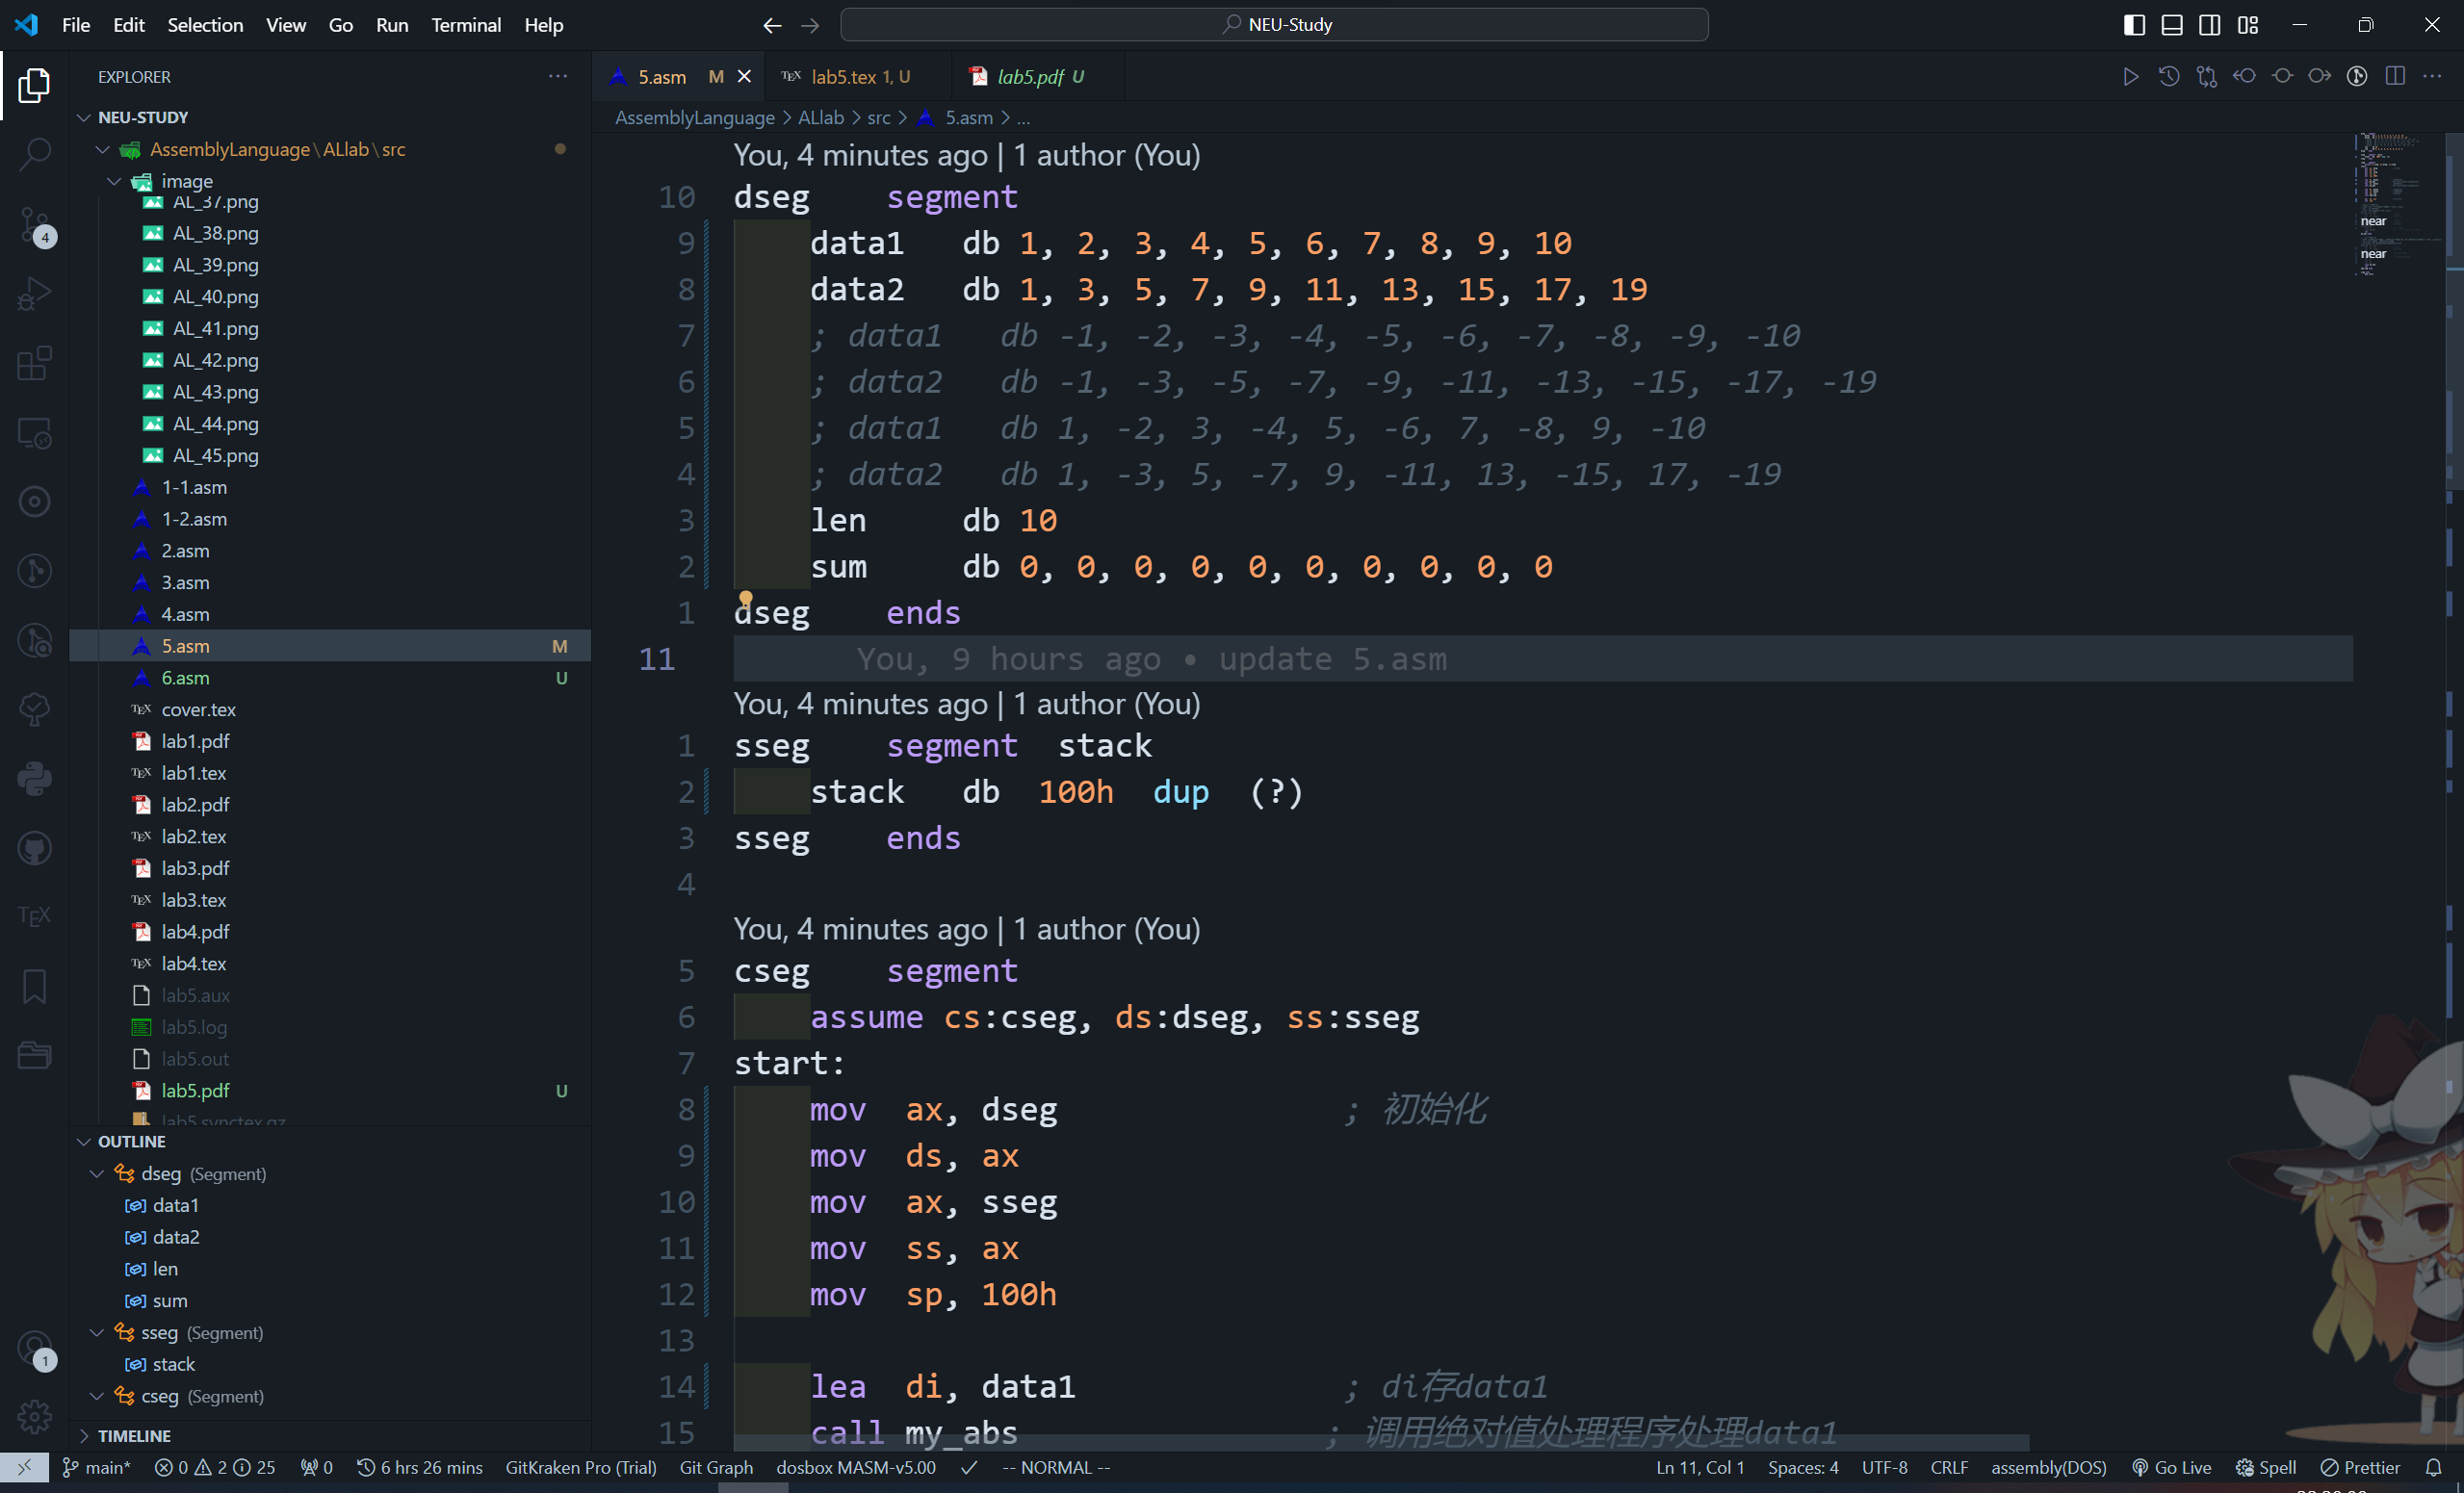
\includegraphics[width=1\textwidth]{image/AL_46.png}\end{center}
    \begin{center}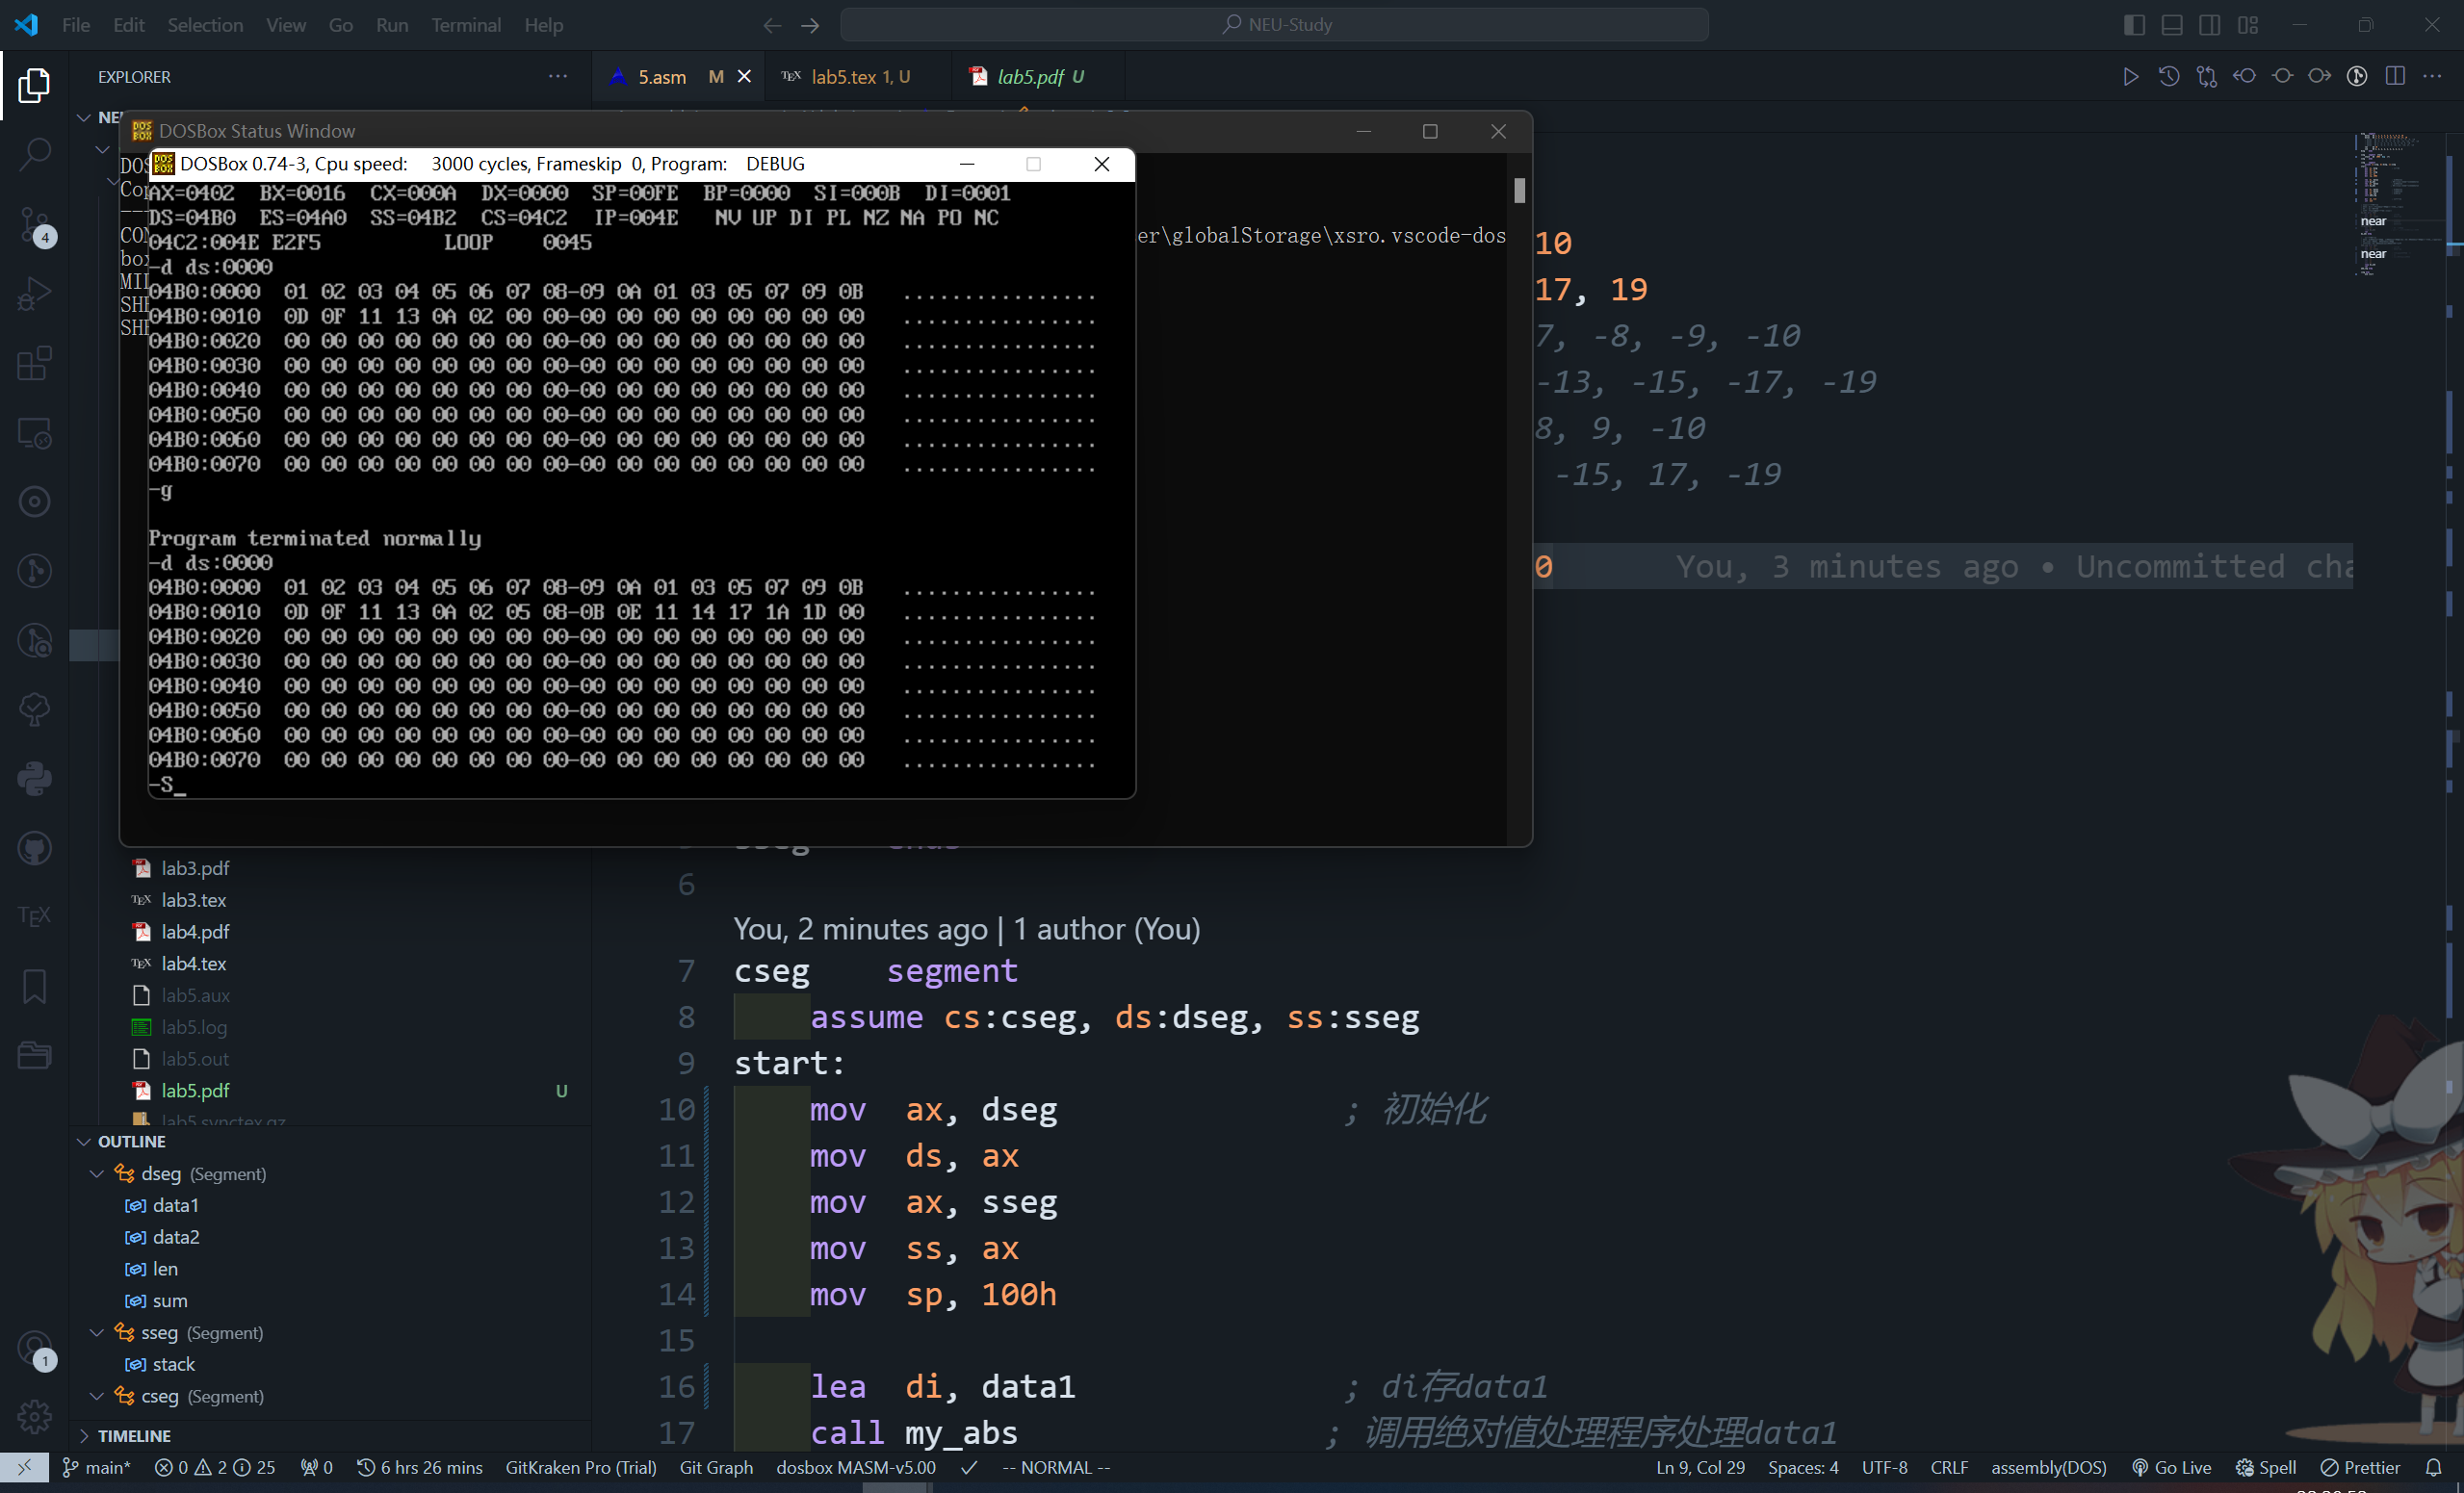
\includegraphics[width=1\textwidth]{image/AL_47.png}\end{center}
    两个多字节数据都是负数
    \begin{center}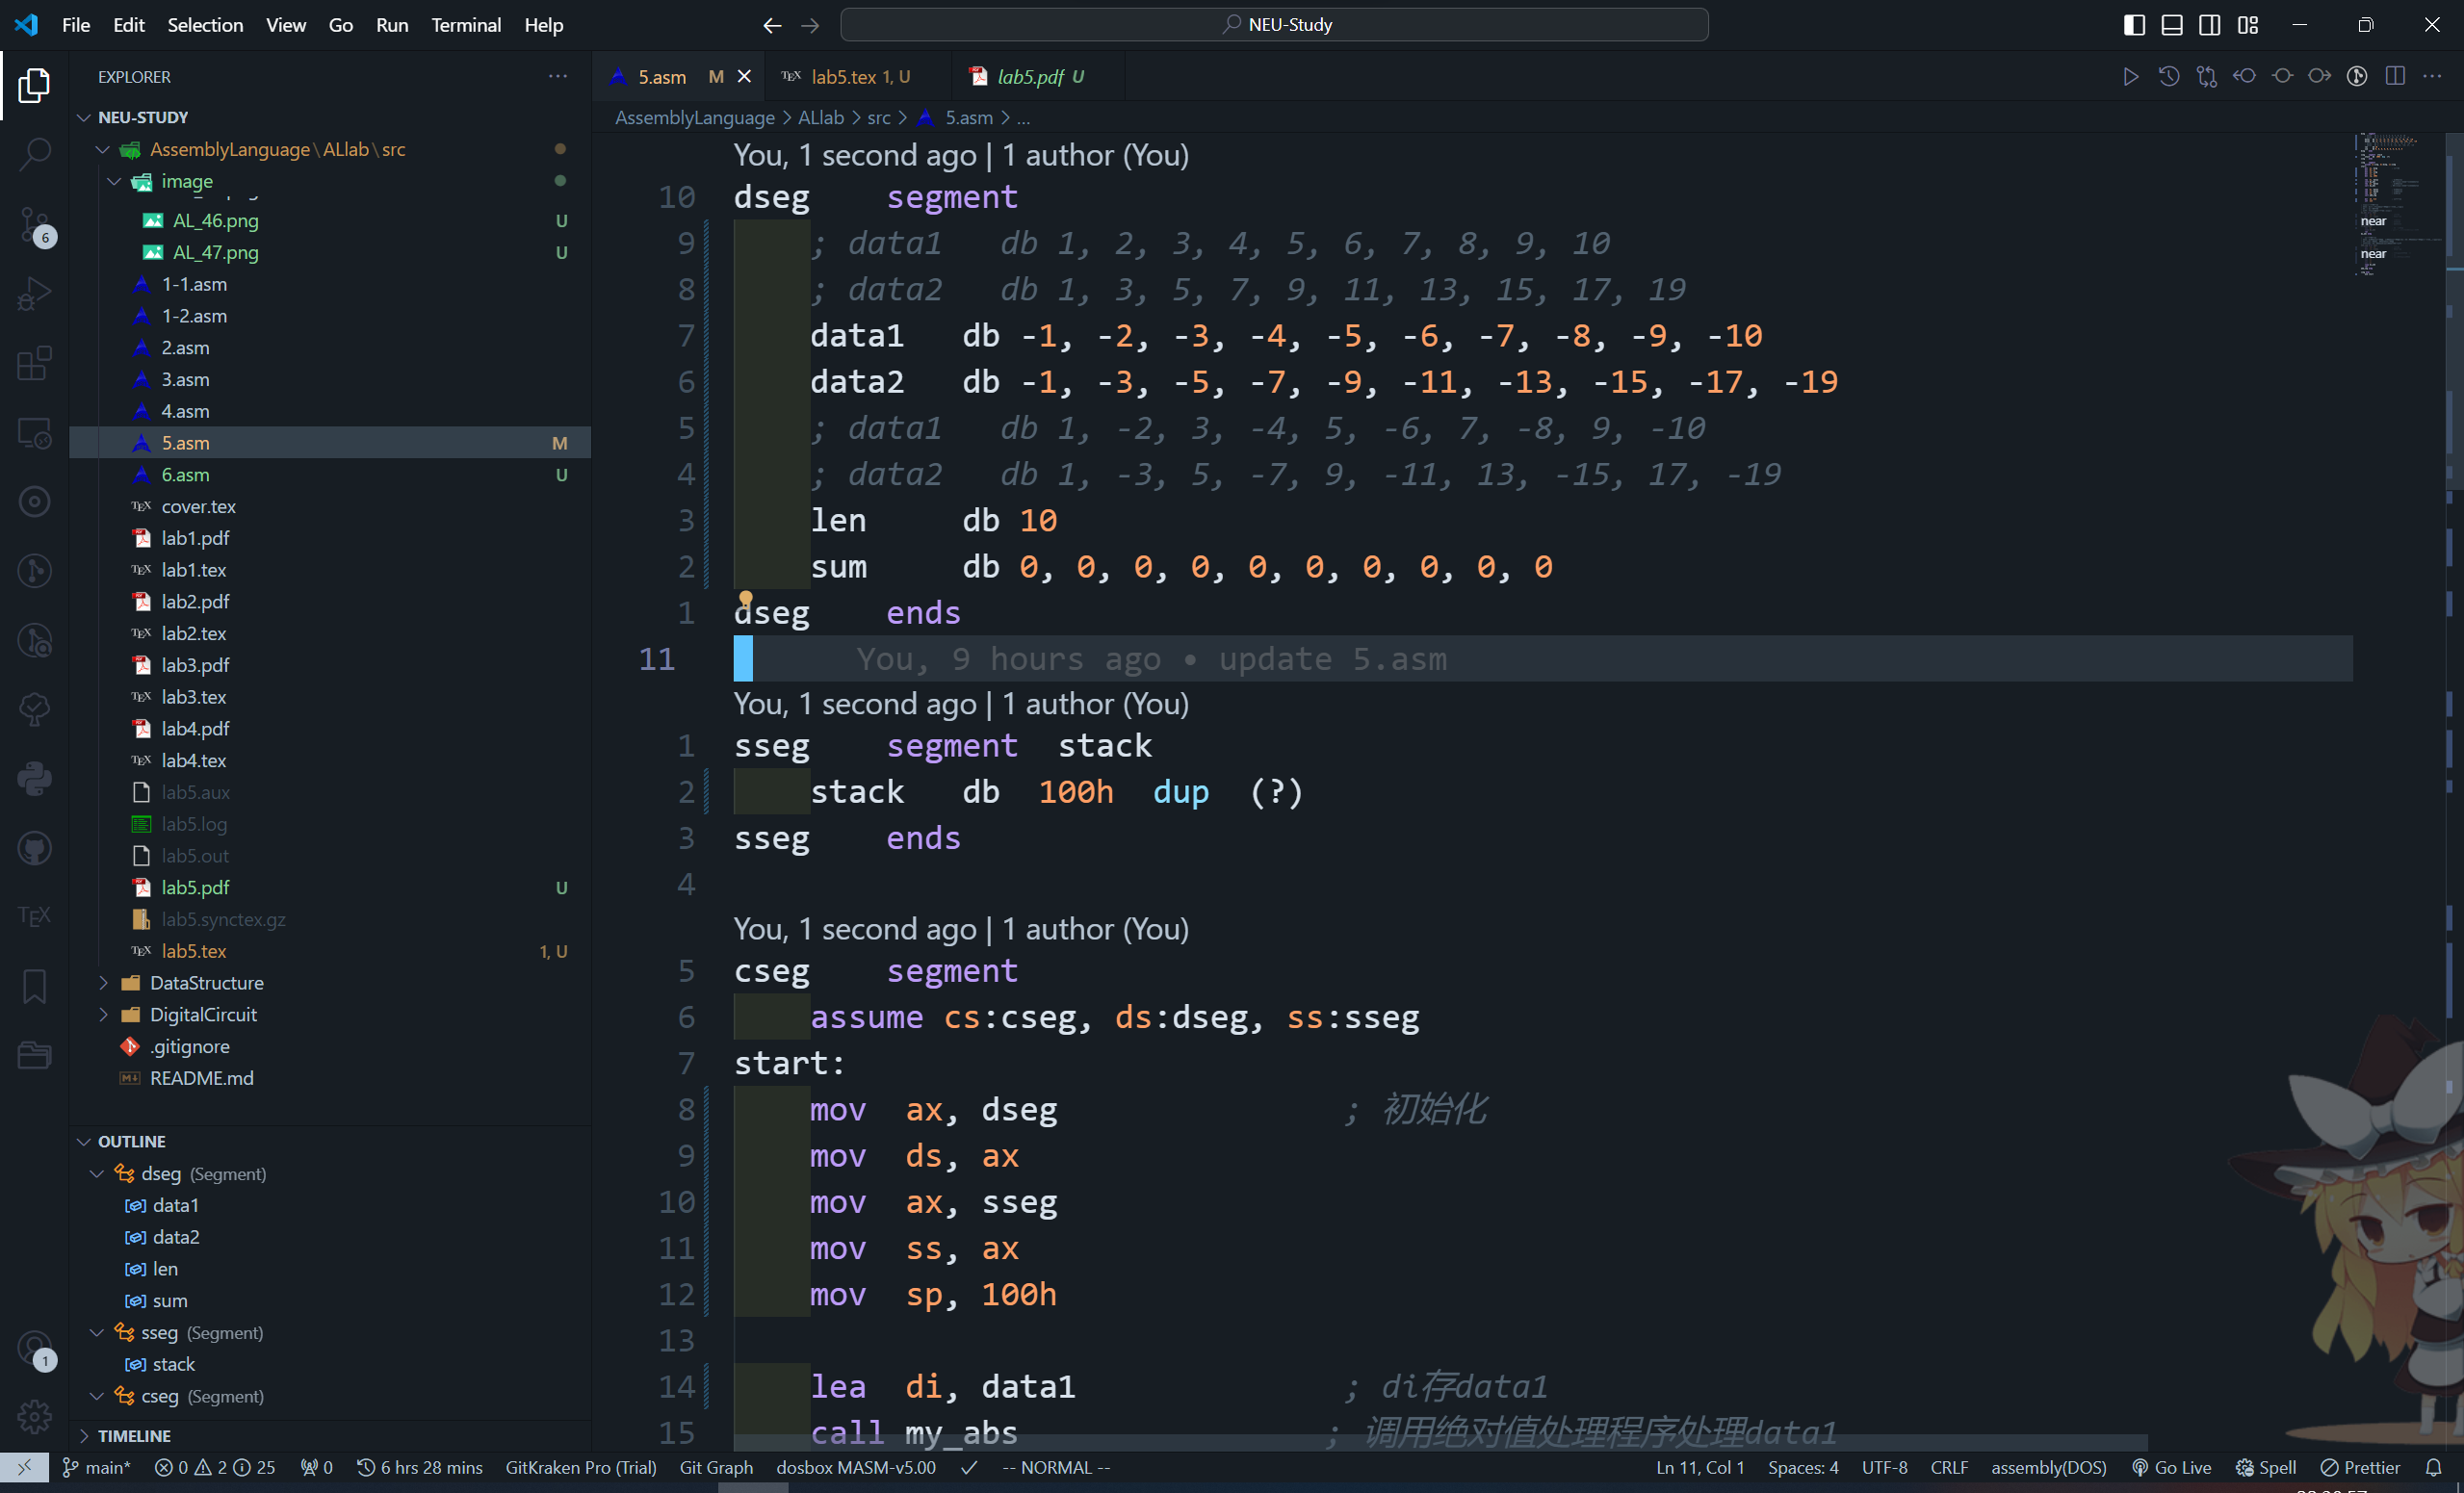
\includegraphics[width=1\textwidth]{image/AL_48.png}\end{center}
    \begin{center}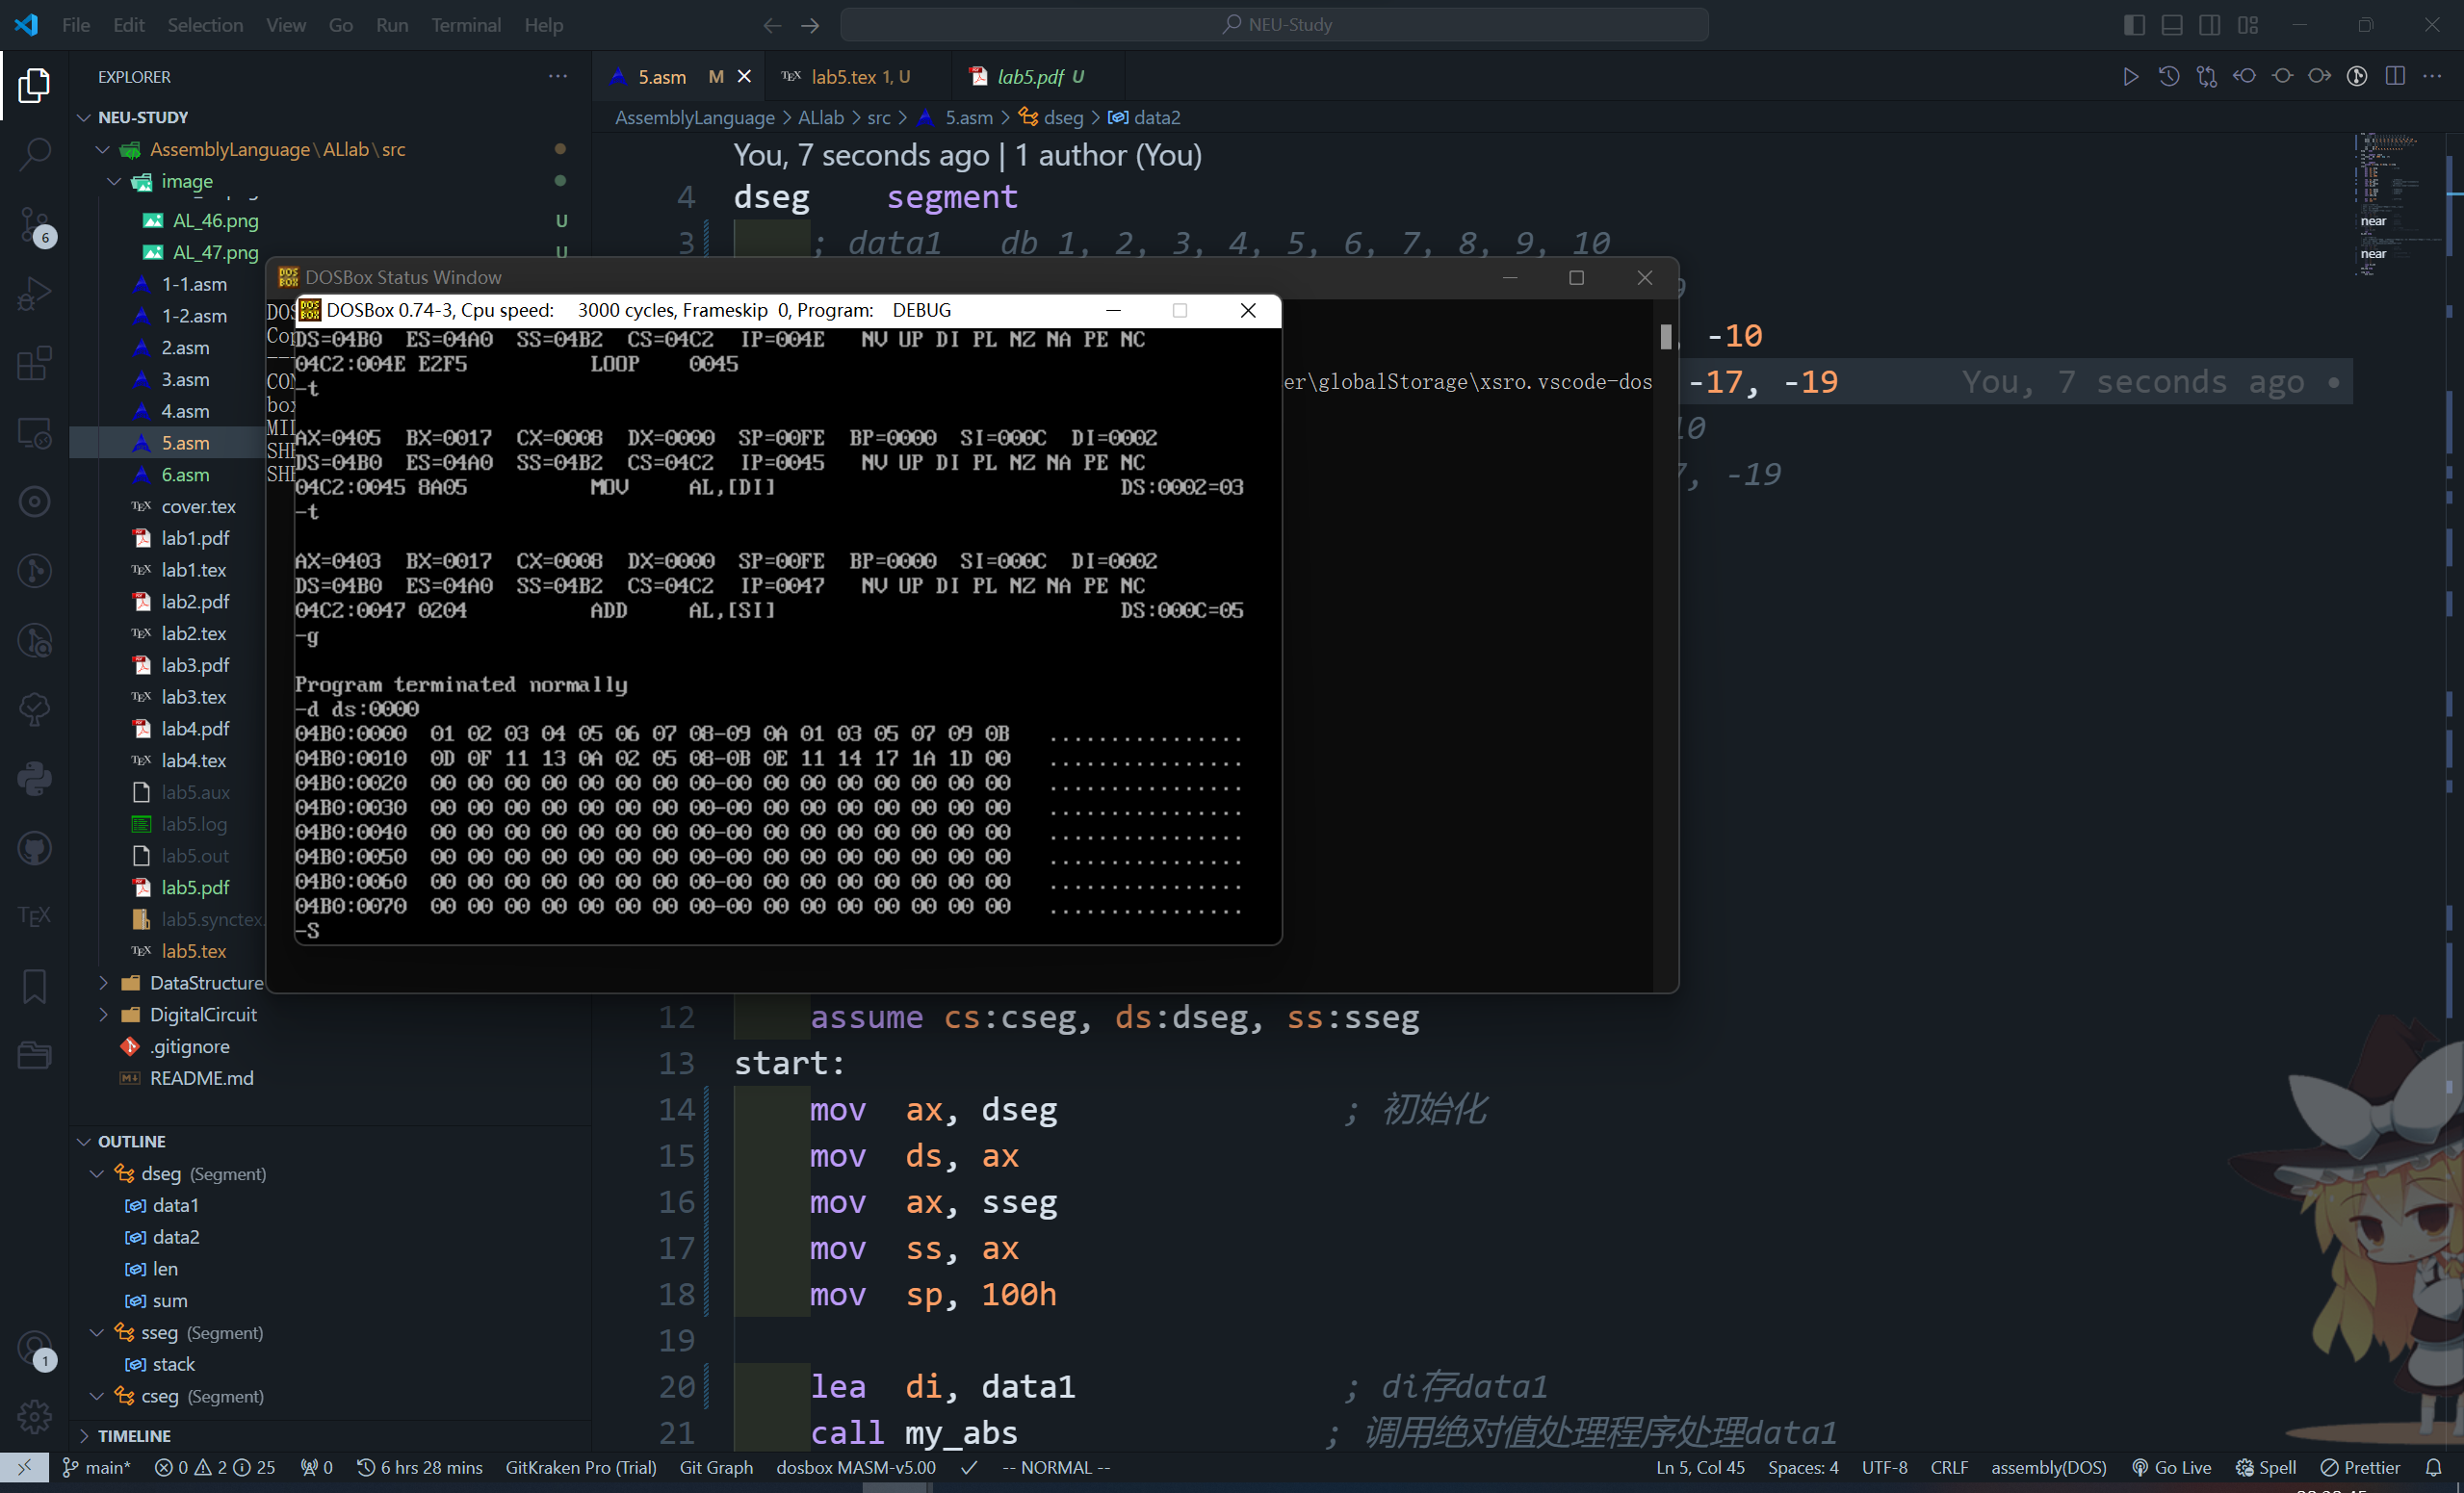
\includegraphics[width=1\textwidth]{image/AL_49.png}\end{center}
    两个多字节数据一正一负：
    \begin{center}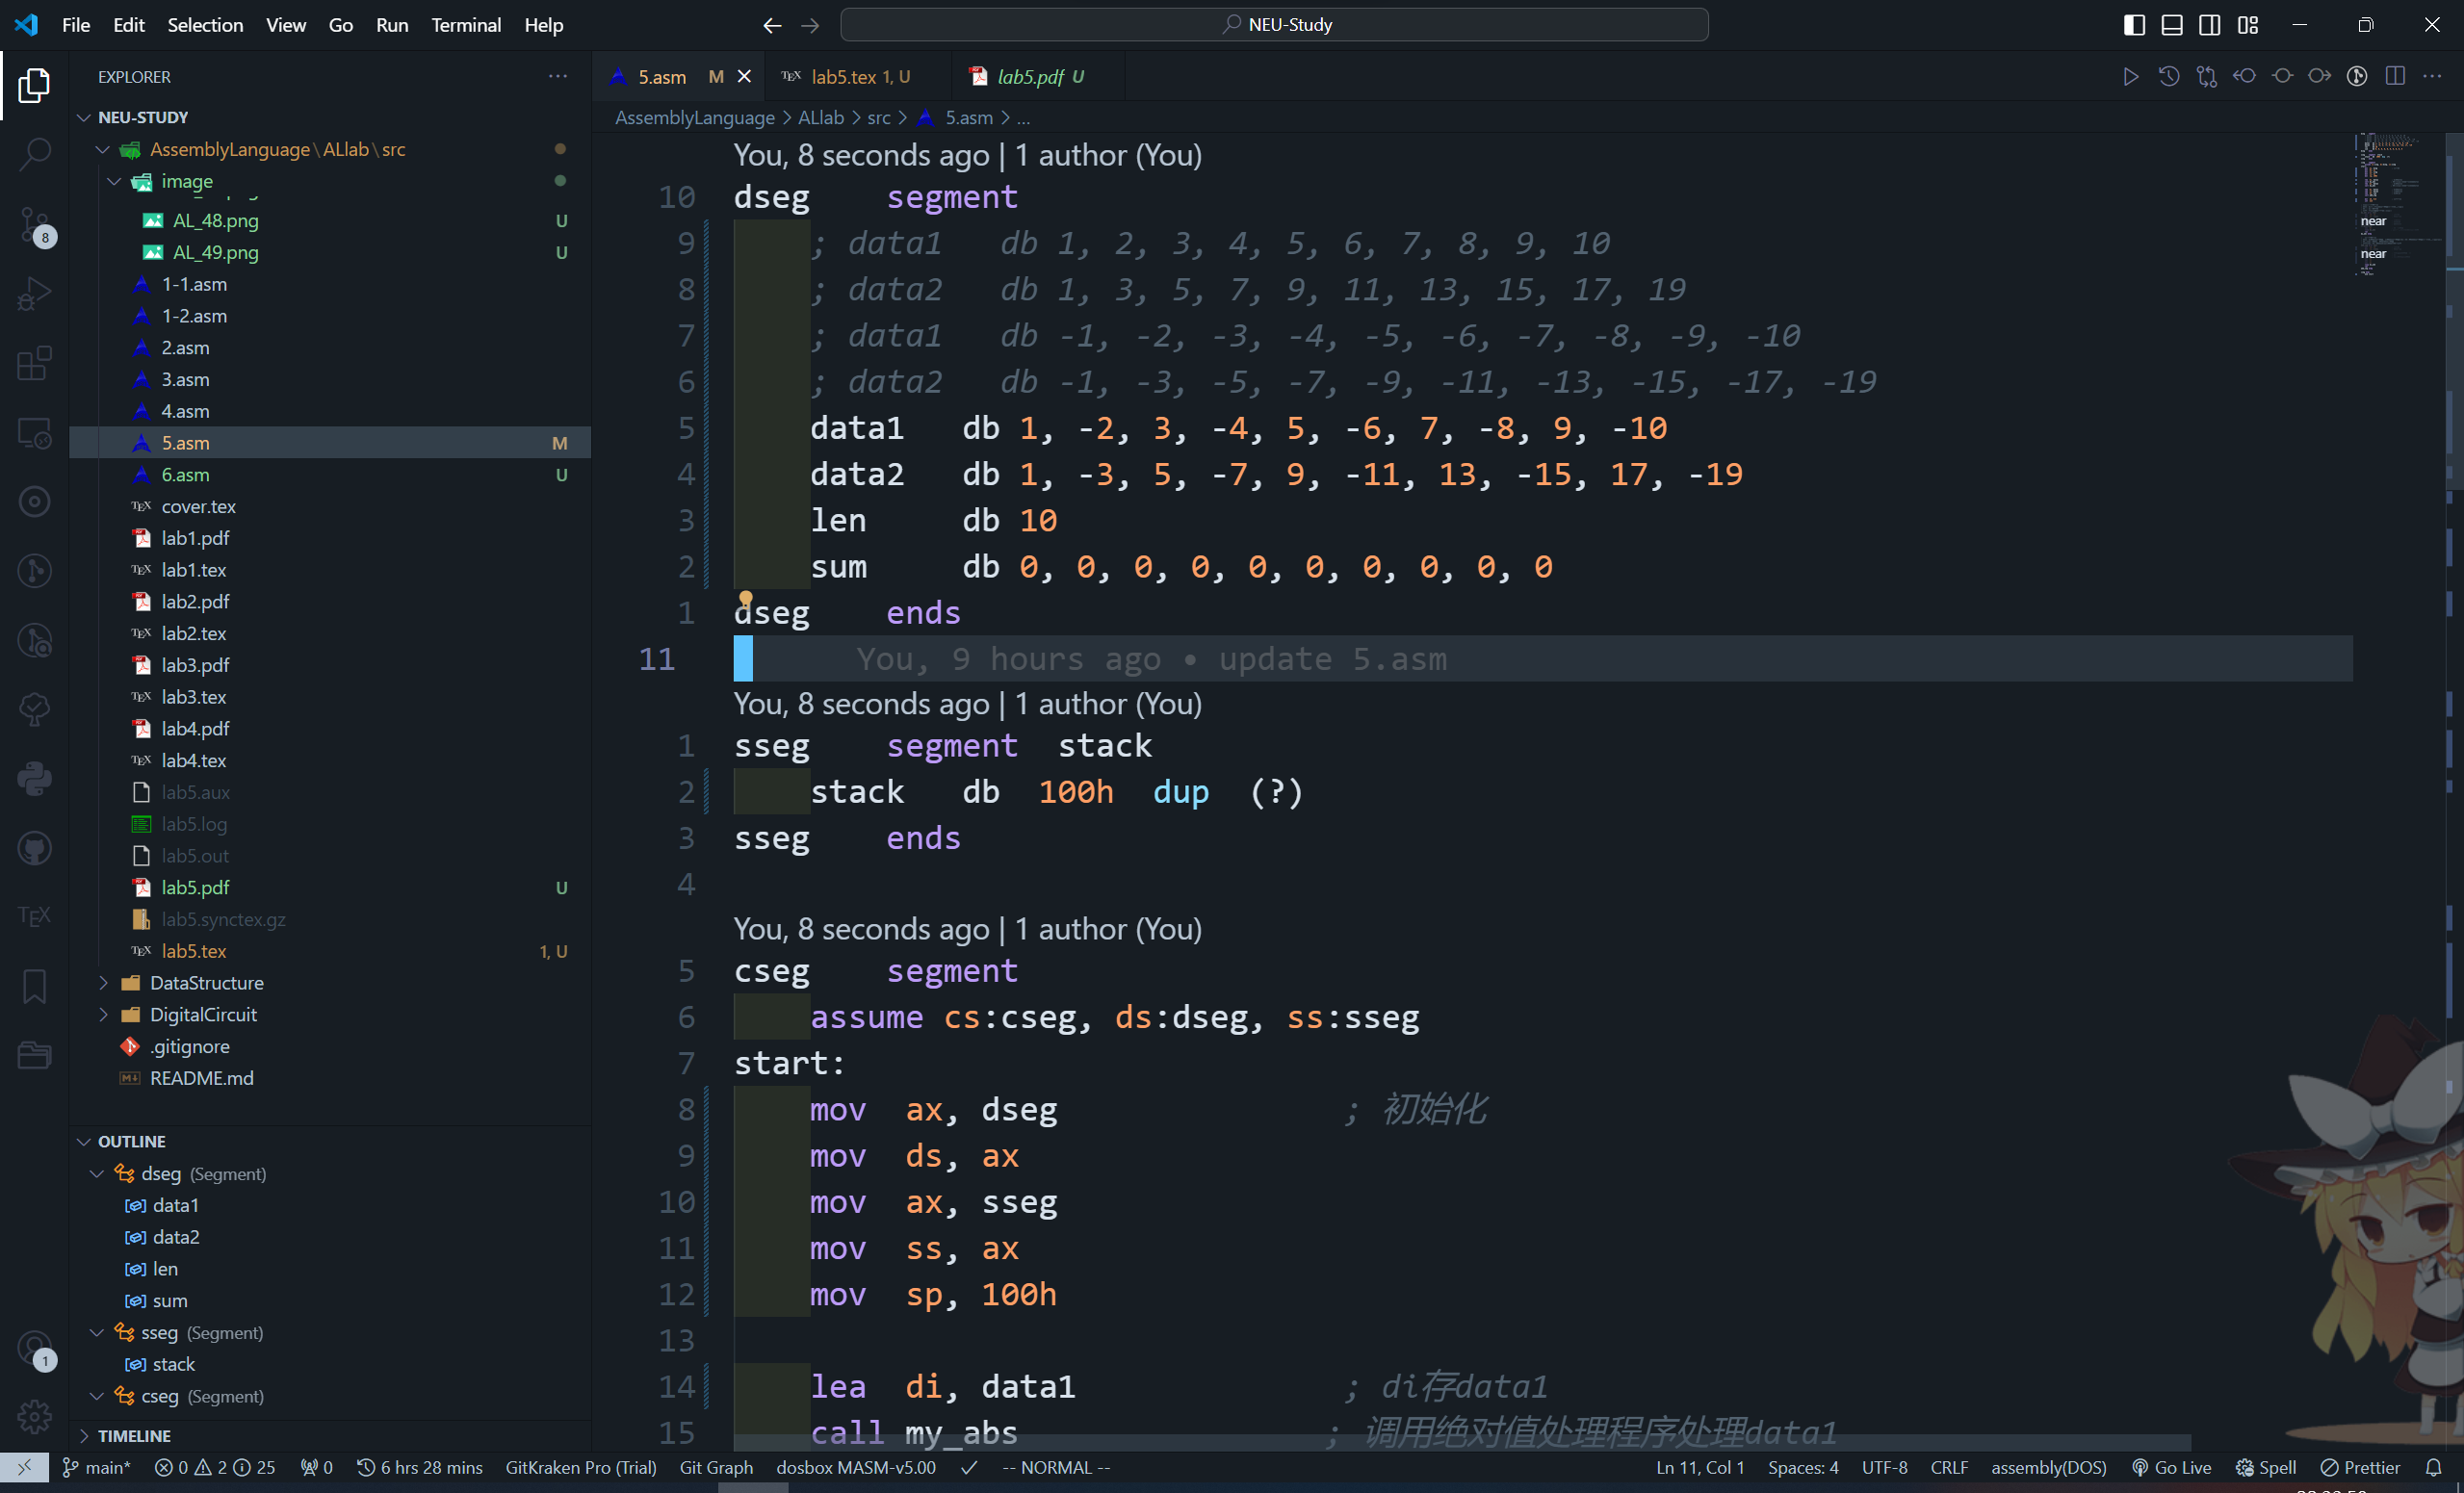
\includegraphics[width=1\textwidth]{image/AL_50.png}\end{center}
    \begin{center}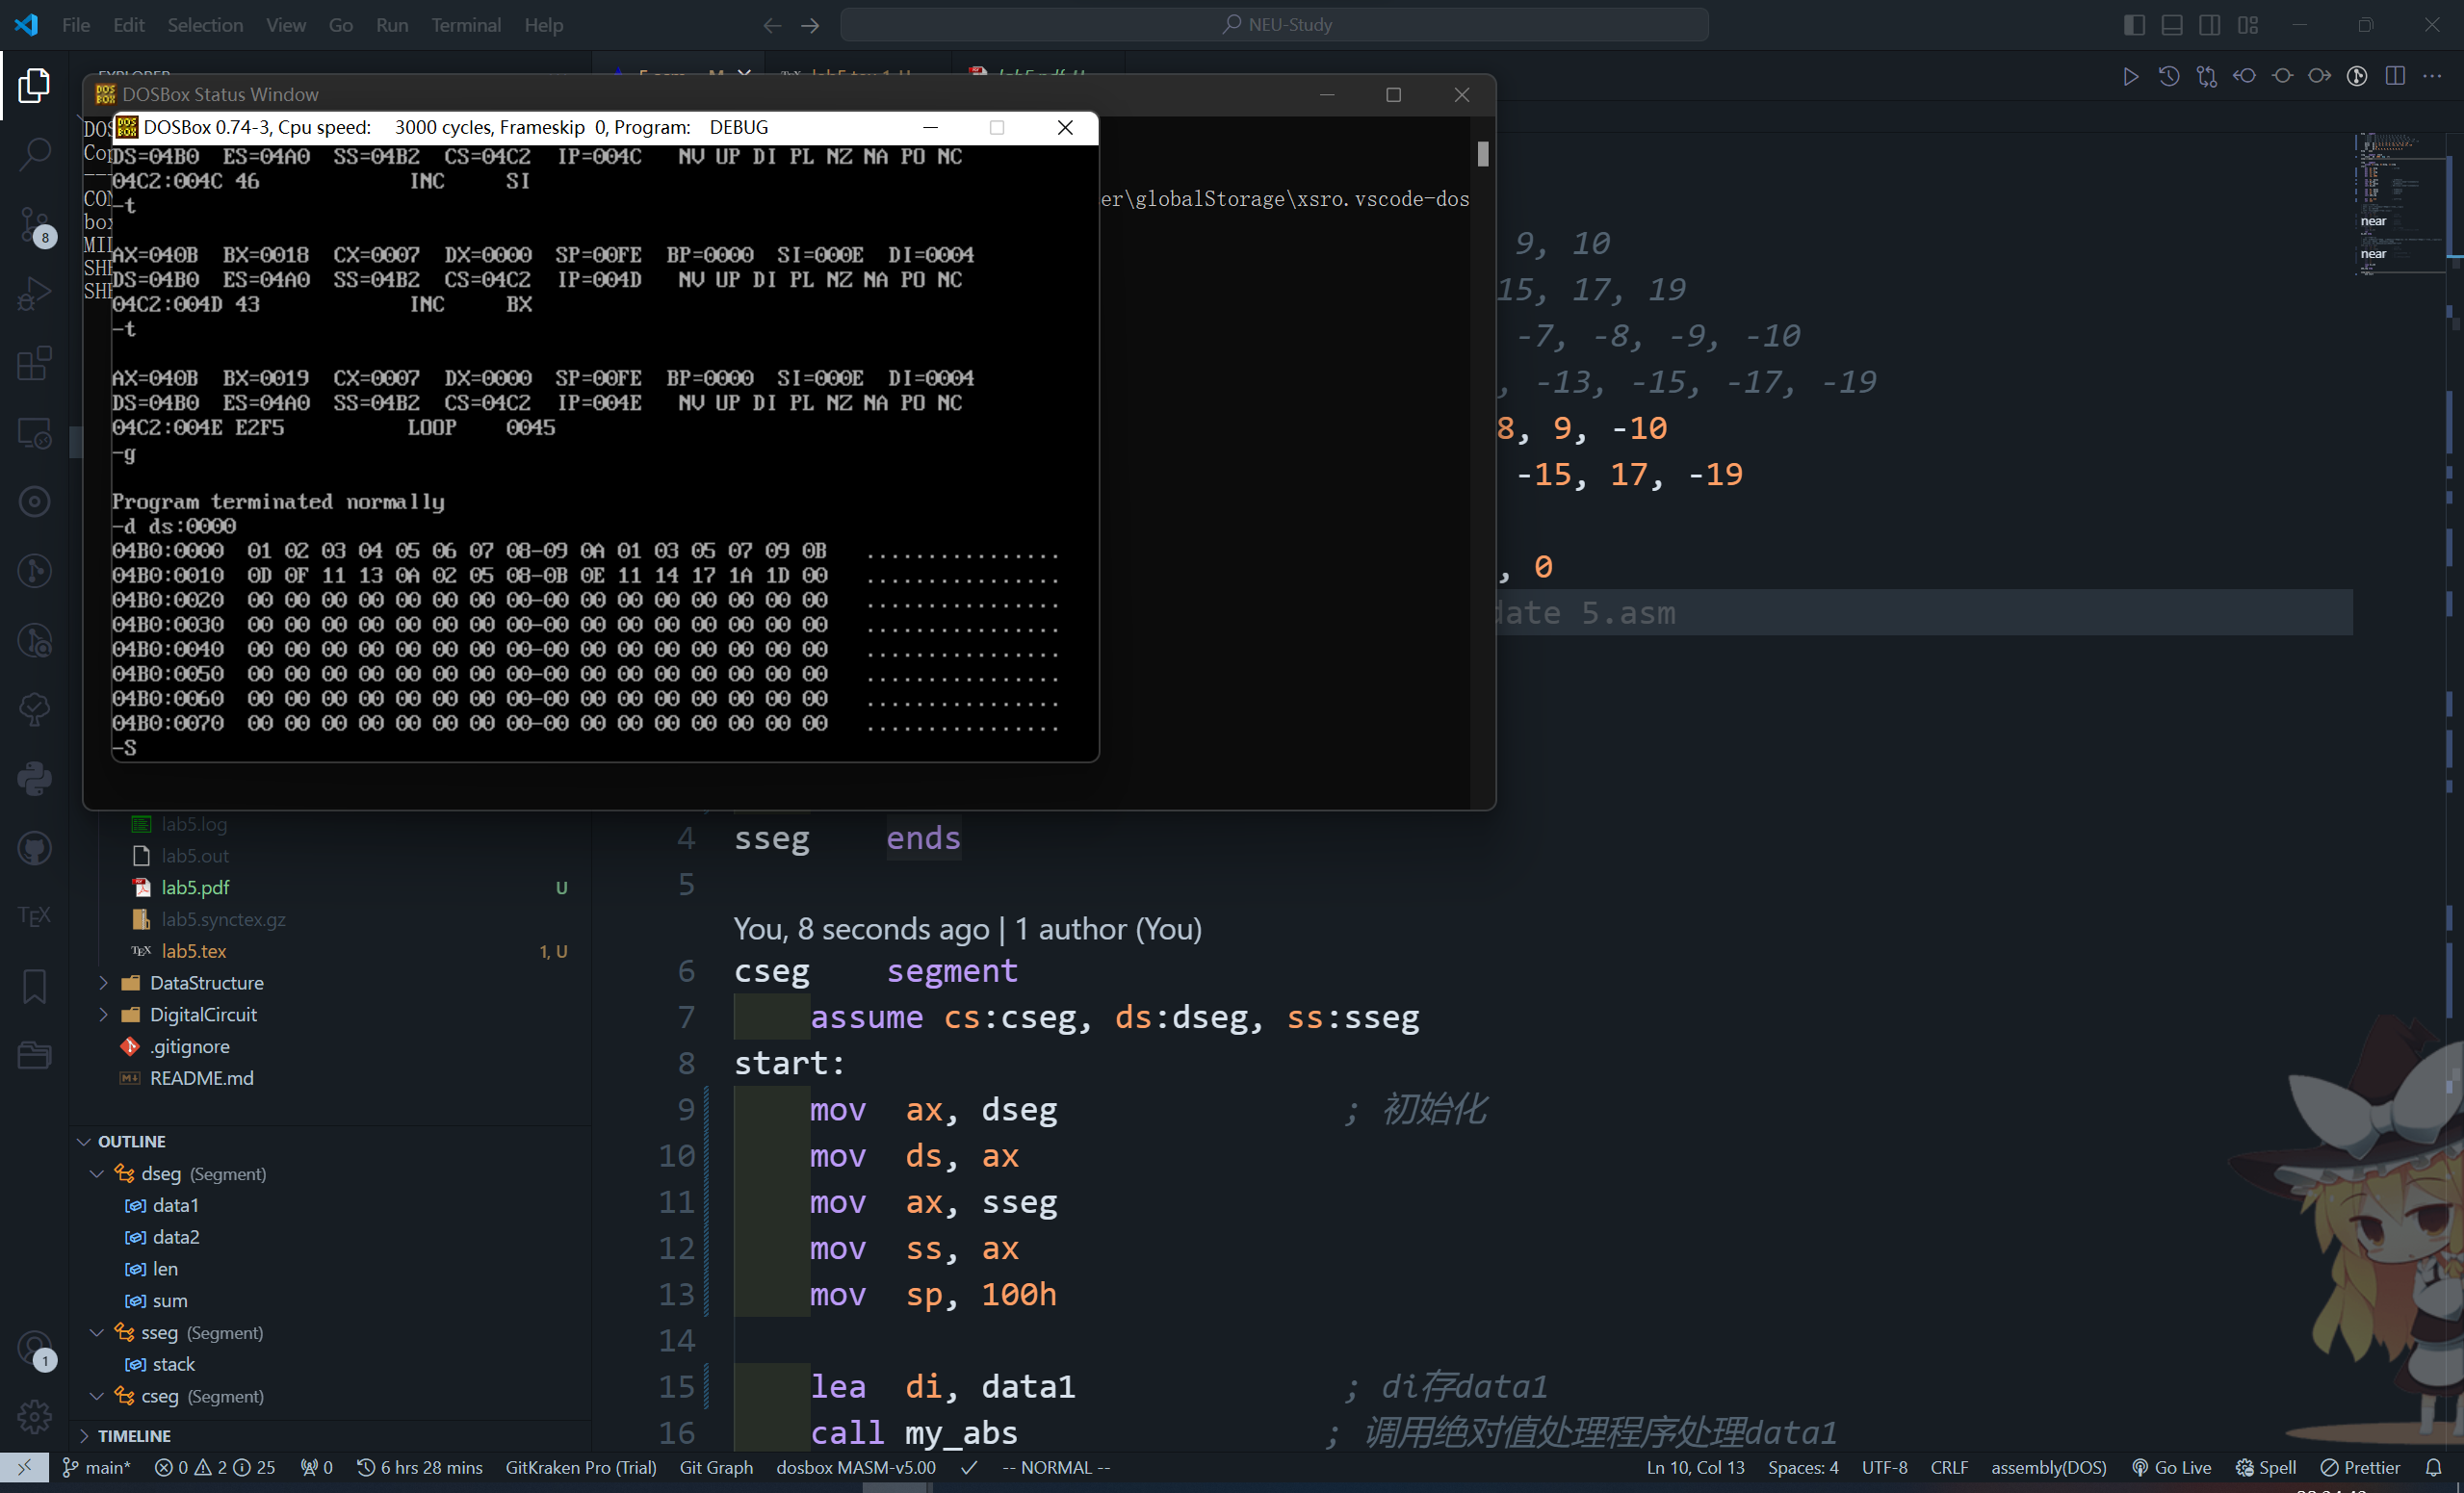
\includegraphics[width=1\textwidth]{image/AL_51.png}\end{center}
    \subsection{流程图}
    \begin{center}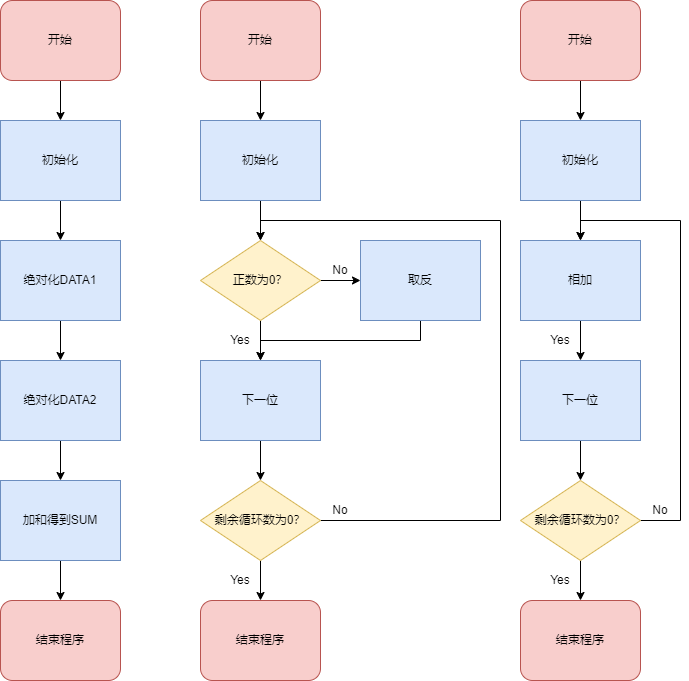
\includegraphics[width=1\textwidth]{image/AL_52.png}\end{center}

\section{心得体会}
通过本次汇编语言的实验，我获得了许多关于程序设计、子程序实现和汇编语言特有功能的实践经验。
本次实验不仅加深了我对汇编语言编程的理解，也增强了我的问题解决能力。

我学习到了如何有效地设计和实现子程序来处理特定的任务，例如计算绝对值和执行加法操作。
通过将复杂功能分解成更小的模块，我能更好地管理和维护代码。

在进行数据处理时，对于地址寄存器的操作尤其重要。
本次实验让我对DI、SI、BX等寄存器的使用有了更深入的理解，尤其是它们在数组处理和数据传递中的作用。

通过本次实验，我对各种汇编指令如LOOP、JGE、NEG等的应用场景和执行效果有了更全面的认识。

汇编语言的调试比高级语言更为复杂，因为错误可能不会直接表现出来。
在调试过程中，我学会了使用仿真工具进行逐步跟踪和检查寄存器的值，这极大地帮助我理解程序的运行过程和发现错误所在。

最初在子程序之间传递数据时遇到困难，特别是在保持数据一致性和正确性方面。
通过详细学习和实践，我掌握了使用堆栈以及直接寄存器传递数据的方法。

本次实验是对我的编程技能和逻辑思维能力的一次全面提升。
它不仅提高了我的汇编语言水平，还加深了我对程序结构设计和模块化编程的理解。
通过实际编写和测试程序，我感受到了理论知识与实践应用之间的联系，这对我的学术和职业发展都具有重要意义。

这次实验让我认识到了汇编语言的强大与精细，以及在现代编程实践中运用这些底层知识的重要性。
我期待在未来的学习和研究中，将这些经验应用到更复杂的问题解决中去。
\begin{flushright}\begin{tabular}{rl}
    姓名: & 李俊洁\\
    班级: & 计算机2204 \\
    学号: & 20225443 \\
    课程: & 汇编语言程序设计 \\
    日期: & April 17, 2024 \\
    制作: & \LaTeX \\
    & 感谢您的批阅！
\end{tabular}\end{flushright}
\end{document}